\section{Peer-to-Peer-Technologie}
\label{subsec:peer_to_peer_technologie}

Peer-to-Peer-Technologien können in zwei Kategorien unterteilt werden: \textit{Peer-to-Peer-Anwendungen} und \textit{Peer-to-Peer-Infrastrukturen} \parencite[S. 730]{Khatibi_StructuredUnstructuredP2P}. 

Die Kategorie der Peer-to-Peer-Anwendungen umfasst den Dienst der \textit{Inhaltsverteilung}, bei dem die Teilnehmer Inhalte wie Musik, Videos oder andere Dateien direkt untereinander austauschen \Parencite[730-731]{Khatibi_StructuredUnstructuredP2P}. 

Daher werden viele Peer-to-Peer schnell mit Filesharing in Verbindung bringen, da diese Technologie in der Vergangenheit vor allem dafür genutzt wurde. Das bekannteste Beispiel ist das Filesharing-Netzwerk \textit{Napster}, das 1999 von Shawn \enquote{Napster} Fanning entwickelt wurde. \textit{Napster} war das erste weit verbreitete Filesharing-Netzwerk, das auf Peer-to-Peer-Technologie basierte. Es ermöglichte den Austausch von Musikdateien zwischen den Teilnehmern. Die Musikdateien wurden dabei auf den Computern der Teilnehmer gespeichert und konnten von anderen Teilnehmern heruntergeladen werden. Da diese Art des Datenaustauschs oftmals illegal war, wurde Napster 2001 aufgrund von Urheberrechtsverletzungen abgeschaltet \parencite[S. 55-57]{Mahlmann_P2PNetzwerke}.

Die zweite Kategorie ist die Peer-to-Peer-Infrastruktur, welche die Peer-to-Peer-Netz-\\werke umfasst, die für die Kommunikation zwischen den Teilnehmern des Netzwerks verwendet werden \parencite[S. 730-731]{Khatibi_StructuredUnstructuredP2P}. Hier sind alle Teilnehmer und fungieren sowohl als Client als auch als Server. Es gibt keine zentrale Instanz, die die Kommunikation steuert. Die Teilnehmer sind direkt miteinander verbunden und können Nachrichten oder andere Daten direkt austauschen.

Diese Art von Peer-to-Peer-Netzwerken wird in dieser Arbeit behandelt.

Im Bereich des Instant Messaging stellt das Peer-to-Peer-Modell eine dezentrale Struktur dar, die die Kommunikation zwischen den Nutzern eines Instant-Messaging-Dienstes ermöglicht. Im Gegensatz zum Client-Server-Ansatz, bei dem ein zentraler Server die Kommunikation steuert, ermöglicht das Peer-to-Peer-Netzwerk eine direkte Kommunikation zwischen den Teilnehmern. Beide Modelle haben ihre Vor- und Nachteile. Während das Client-Server-Modell eine zentrale Instanz erfordert, um die Kommunikation zu verwalten, ist das Peer-to-Peer-Netzwerk dezentralisiert und benötigt eine solche Instanz nicht. Die Implementierung und Wartung eines Client-Server-Modells sind im Vergleich zu einem komplexeren und aufwendigeren Peer-to-Peer-Netzwerk einfacher. Das Client-Server-Modell ist weniger flexibel, da es von einer zentralen Instanz abhängt, während das Peer-to-Peer-Netzwerk aufgrund des Fehlens dieser Instanz flexibler ist. Ein weiterer Unterschied betrifft die Skalierbarkeit: Das Client-Server-Modell ist durch die Kapazität des Servers begrenzt, während das Peer-to-Peer-Netzwerk auf die Kapazität der Teilnehmer zurückgreift, was seine Skalierbarkeit verbessert. Hinsichtlich der Sicherheit ist das Client-Server-Modell weniger robust, da es auf eine zentrale Instanz angewiesen ist, während das Peer-to-Peer-Netzwerk als sicherer gilt, da es ohne eine solche Abhängigkeit auskommt \parencite[S. 6-8]{Mahlmann_P2PNetzwerke}.


\subsection{Typen von Peer-to-Peer-Netzwerken}

Nicht jedes Peer-to-Peer-Netzwerk ist gleich aufgebaut. Es gibt verschiedene Typen von Peer-to-Peer-Netzwerken, die sich in ihrer Struktur und Funktionsweise unterscheiden. Abbildung \ref{p2p_typen} zeigt die zwei Haupttypen von Peer-to-Peer-Netzwerken: unstrukturierte und strukturierte Netzwerke \parencite[S. 362-363]{Luntovskyy_ModRechnernetze}.

\begin{center}
    \captionsetup{type=figure}
    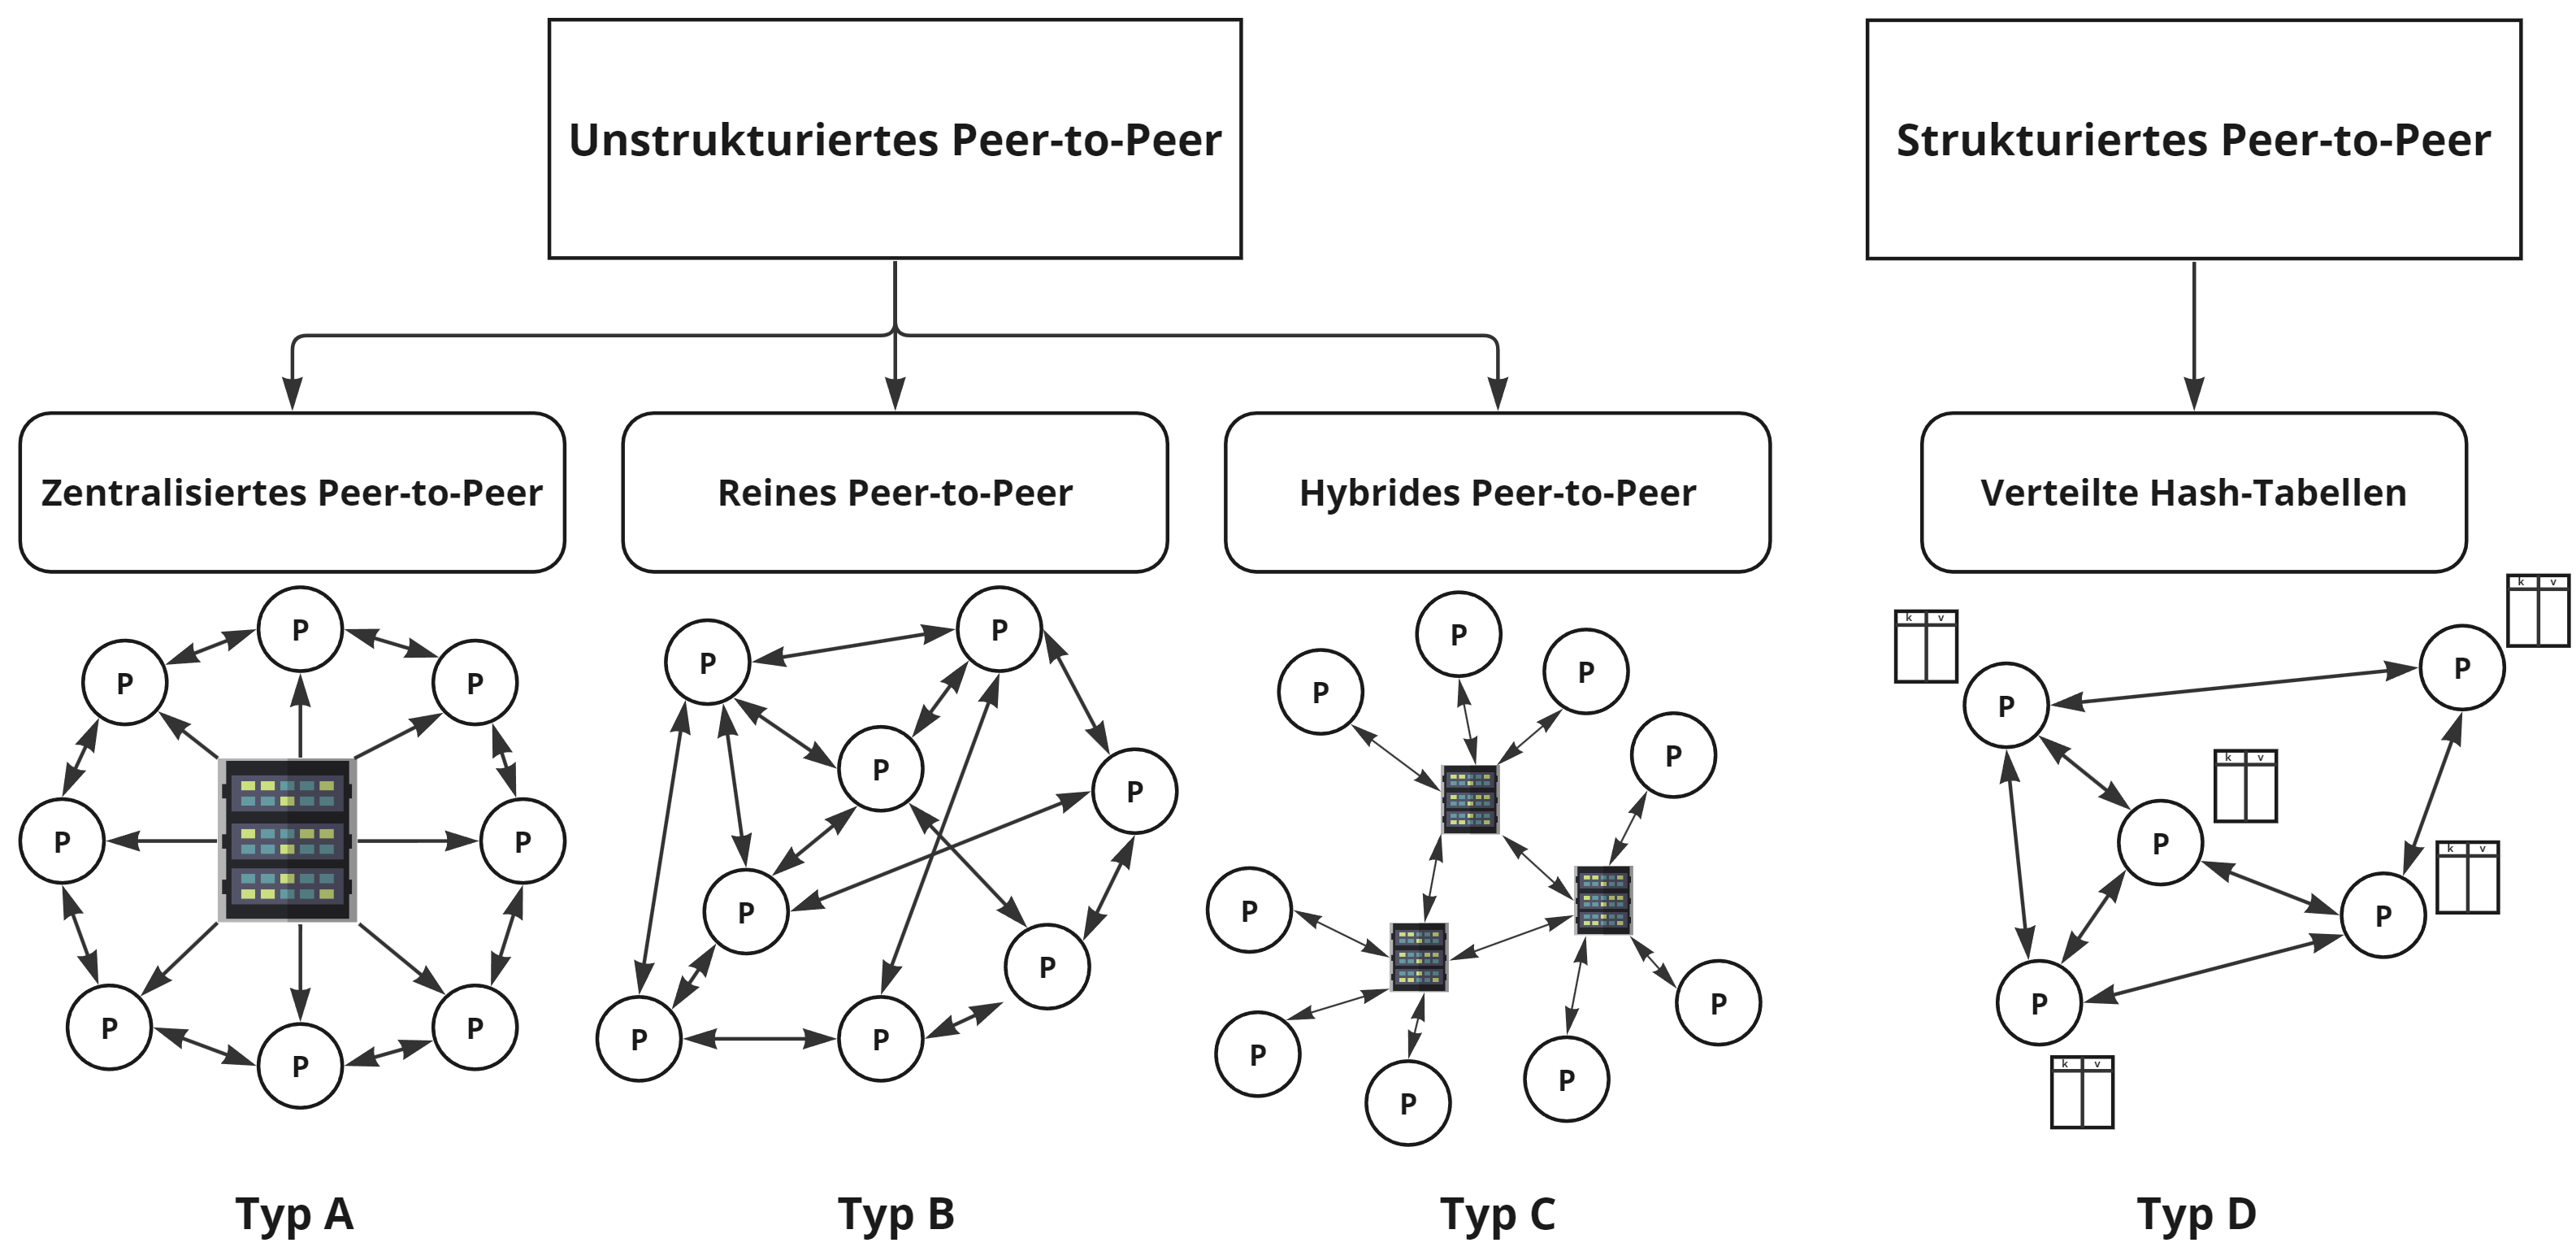
\includegraphics[width=1\linewidth]{images/p2p_typen.png}
    \captionof{figure}{Typen von Peer-to-Peer-Netzwerken (in Anlehnung an \cite[S. 363]{Luntovskyy_ModRechnernetze})}
    \label{p2p_typen}
\end{center}

\noindent Unstrukturierte und strukturierte Peer-to-Peer-Netzwerke sind unterschiedliche Ansätze zur Organisation von Knoten (engl. \textit{Nodes}) und Ressourcen in dezentralen Netzwerken.

Unstrukturierte Netzwerke sind charakterisiert durch ihre fehlende explizite Organisationsstruktur, was eine einfache Konnektivität ermöglicht. \textit{Typ A} in Abbildung \ref{p2p_typen} zeigt ein zentralisiertes Netzwerk, was bedeutet, dass alle Teilnehmer mit einem zentralen Server verbunden sind. Als Beispiel für diese Form des Peer-to-Peer dient \textit{Napster}. Bei \textit{Napster} gab es mehrere Server, die die Dateien der Teilnehmer indizierten. Die Teilnehmer konnten Dateien von anderen Teilnehmern herunterladen, indem sie eine Anfrage an einen der Server stellten, der dann die IP-Adresse des Teilnehmers zurückgab, der die gesuchte Datei zur Verfügung stellte \parencite[S. 171]{Saroiu_MeasuringAndAnalyzingNapsterAndGnutellaHosts}. Diese Form ermöglicht eine schnelle und effiziente Suche nach Ressourcen, da die Ressourcen zentral verwaltet werden, aber die Abhängigkeit von einem zentralen Server macht das Netzwerk nicht skalierbar und anfällig für Ausfälle \parencite[S. 732]{Khatibi_StructuredUnstructuredP2P}.
Bei \textit{Typ B} handelt es sich um ein reines Peer-to-Peer-Netzwerk, bei dem die Teilnehmer direkt miteinander verbunden sind und jeder sowohl als Client als auch als Server fungiert \parencite[S. 732]{Khatibi_StructuredUnstructuredP2P}. Ein Beispiel für diese Form des Peer-to-Peer ist \textit{Gnutella}. Bei \textit{Gnutella} gab es keine zentrale Instanz, die die Ressourcen der Teilnehmer indizierte. Die Suche nach Ressourcen oder Informationen erfolgt durch Broadcasts oder zufällige Weiterleitungen, was jedoch zu ineffizienten Suchprozessen führen kann, da keine klare Routing-Struktur vorhanden ist \parencite[S. 171]{Saroiu_MeasuringAndAnalyzingNapsterAndGnutellaHosts}. Beim dritten und letzten Typ (\textit{Typ C}) der unstrukturierten Netzwerke handelt es sich um ein hybrides Peer-to-Peer-Netzwerk, das Elemente aus den beiden anderen Typen kombiniert. In einem hybriden Netzwerk gibt es besondere Knoten, die die Funktionen eines Servers, wie beispielsweise Indexierung der Ressourcen, für eine bestimmte Gruppe von Teilnehmern übernehmen. Diese Knoten werden als Superknoten (engl. \textit{Super Nodes}) bezeichnet. Die Super Nodes selbst sind untereinander dezentralisiert miteinander verbunden. Ein Beispiel für diese Form des Peer-to-Peer ist \textit{Gnutella2} \parencite[S. 732]{Khatibi_StructuredUnstructuredP2P}. 

Strukturierte Peer-to-Peer-Netzwerke hingegen weisen klare Regeln und Algorithmen zur Organisation der Knoten auf. Diese Netzwerke verfügen über eine explizite Organisationsstruktur, sei es eine Ringstruktur, k-bucket basierte Systeme oder andere, die es ermöglichen, effizientes Routing und eine optimierte Ressourcenverwaltung zu erreichen. Durch diese klar definierte Struktur sind strukturierte Netzwerke oft stabiler und bieten eine effizientere Ressourcenlokalisierung im Vergleich zu ihren unstrukturierten Gegenstücken. Allerdings kann diese Stabilität auf Kosten von Flexibilität und Anpassungsfähigkeit gehen, da Änderungen in der Netzwerktopologie oder hohe Dynamik der Knoten schwerer zu handhaben sind \parencite[S. 40]{Vu_P2PComputing}.


\subsection{Problemstellung und mögliche Lösungen}
\label{subsec:problemstellung_und_moegliche_loesungen}

Leider bringen Peer-to-Peer-Netzwerke auch einige Probleme mit sich. Eines der Probleme stellen die \textit{Network Address Translators} (kurz: \textit{NATs}) dar. NATs sind dafür zuständig, private IP-Adressen in öffentliche IP-Adressen umzuwandeln und umgekehrt. Sie werden in Routern oder Gateways eingesetzt und dienen dazu, den Zugang von Geräten im lokalen Netzwerk, welche private IP-Adressen verwenden, zum Internet zu ermöglichen, indem sie den Datenverkehr zwischen dem lokalen Netzwerk und dem externen Netzwerk, wie dem Internet, verwalten. Peer-to-Peer Verbindungen stoßen bei Network Address Translators oft auf Probleme, was daran liegt, dass NATs normalerweise nicht erlauben, dass externe Geräte direkt mit internen Geräten kommunizieren. Zudem werden Ports dynamisch für ausgehenden Traffic zugewiesen, was das Weiterleiten eingehender Verbindungen erschwert. Symmetrische NATs verschärfen dieses Problem, da sie für ausgehende Verbindungen eine eindeutige Kombination von IP-Adresse und Port verwenden, die sich bei jeder neuen Verbindung ändert \Parencite[S. 1-9]{rfc2663_NAT_Terminology}.

NATs stellen also eine große Herausforderung für Peer-to-Peer-Netzwerke dar, da sie die direkte Kommunikation zwischen den Teilnehmern erschweren, wenn sie sich hinter einem NAT befinden. Um dieses Problem zu lösen, gibt es verschiedene Lösungsansätze. Einer davon ist das \textit{Relaying}. Das Verb \textit{to relay} kann mit \textit{weiterleiten} oder \textit{weitergeben} übersetzt werden. Beim Relaying wird also ein Server als Vermittler zwischen den Teilnehmern verwendet, der die Nachrichten zwischen den Teilnehmern weiterleitet. Damit sich die Teilnehmer mit dem Server verbinden können, muss dieser eine öffentliche IP-Adresse haben, die jedem Teilnehmer bekannt ist. Dieser Ansatz ist einfach zu implementieren, erfordert aber einen zentralen Server, der diese Aufgabe übernimmt. Zudem ist er nicht sehr effizient, da der Server die Nachrichten zwischen den Teilnehmern weiterleiten muss, was zu einer höheren Latenz führen kann. Dazu kommt, dass ein solcher Server einen \textit{Single Point of Failure} oder zu Deutsch \textit{einzelner Ausfallpunkt} darstellt, da die Kommunikation zwischen den Teilnehmern unterbrochen wird, wenn der Server ausfällt.

Ein weiterer Ansatz ist die \textit{Connection Reversal}. Bei der Connection Reversal wird ein \textit{Rendezvous-Server} verwendet, um eine Verbindung zwischen den Teilnehmern herzustellen. Der Teilnehmer, der sich im öffentliche Netzwerk befindet, möchte eine Verbindung mit dem Teilnehmer herstellen, der sich hinter dem NAT befindet. Der Aufbau einer direkten Verbindung ist fehlgeschlagen, weshalb der Teilnehmer eine Verbindung mit dem Rendezvous-Server herstellt. Mit Hilfe des Rendezvous-Servers teilt der Teilnehmer im öffentlichen Netzwerk dem Teilnehmer hinter dem NAT seine öffentliche IP-Adresse und Port mit, sodass dieser den Verbindungsaufbau einleitet. Bei dieser Technik darf sich jedoch nur einer der Teilnehmer hinter einem NAT befinden.

\textit{Hole Punching} beschreibt einen weiteren Lösungsansatz. Zwei Geräte, die eine direkte Verbindung miteinander aufbauen möchten, initiieren gleichzeitig eine Verbindung zu einem Server, der sich außerhalb des NATs befindet. Der Server sammelt die IP-Adressen und Ports der beiden Geräte und leitet diese an die jeweils andere Partei weiter. Die beiden Geräte versuchen dann, eine Verbindung zueinander herzustellen, indem sie gleichzeitig Datenpakete an die IP-Adresse und den Port des anderen Geräts senden. Dabei wird versucht, das NAT dazu zu bringen, die Verbindung zu öffnen, indem es die ankommenden Pakete als Antwort auf die ausgehenden Pakete erkennt. Wenn dies gelingt, wird ein temporäres Loch im NAT geöffnet, das es den Geräten ermöglicht, direkt miteinander zu kommunizieren. Diese Technik erfordert eine präzise Koordination und die Fähigkeit der beiden Geräte zur gleichen Zeit Datenpakete zu senden und zu empfangen. Zudem ist es nicht immer möglich, ein temporäres Loch im NAT zu öffnen, da es von der Implementierung des NATs abhängt. 

Eine Abwandlung vom Hole Punching ist die \textit{Port Number Prediction}. Hierbei wird versucht, die Portnummer vorherzusagen, die das NAT für die Verbindung verwenden wird. Durch Beobachtung und Analyse vorheriger Verbindungen wird versucht Muster oder Trends in der Art und Weise zu erkennen, wie Portnummern zugewiesen werden. Dies könnte auf bestimmte Algorithmen oder Verhaltensweisen des Systems hinweisen, woraus dann die Portnummer vorhergesagt werden kann. Diese Technik ist jedoch nicht immer zuverlässig, da es rein auf Annahmen basiert und das Risiko besteht, dass sich das Portzuweisungsmuster jederzeit ändern könnte \Parencite[S. 7-21]{rfc5128_P2P_NATs}.

Um diese Problematik von Peer-to-Peer-Netzwerken zu lösen, können verschiedene Protokolle zum Einsatz kommen. Eines dieser Protokolle ist \textit{STUN} (kurz für \textit{Session Traversal Utilities for NAT}). STUN ist ein Netzwerkprotokoll, das es Geräten, die sich hinter einem NAT befinden, ermöglicht, ihre öffentliche IP-Adresse und Port zu ermitteln. Es bietet an sich keine Möglichkeit für eine Umgehung des NATs, sondern ist dafür gedacht, als eines von mehreren Werkzeugen verwendet zu werden, um ein NAT zu umgehen. Mittels STUN lässt sich nur ermitteln, ob sich ein Gerät hinter einem NAT befindet und wenn dies zutrifft, welche IP-Adresse und Port es verwendet \parencite[S. 4]{rfc8489_STUN}.

\textit{TURN} (kurz für \textit{Traversal Using Relays around NAT}) ist ein weiteres Netzwerkprotokoll, das im Zusammenhang mit NATs verwendet werden kann. Aus der Spezifikation ist zu entnehmen, dass TURN ein Protokoll ist, das es Geräten, die sich hinter einem NAT befinden, ermöglicht, eine Verbindung zu einem anderen Gerät herzustellen, indem es einen Server als Vermittler verwendet (siehe weiter oben in \ref{subsec:problemstellung_und_moegliche_loesungen} \nameref{subsec:problemstellung_und_moegliche_loesungen}). Das funktioniert auch, wenn sich beide Geräte hinter einem NAT befinden \parencite[S. 7]{rfc8656_TURN}.

\textit{ICE} (kurz für \textit{Interactive Connectivity Establishment}) ist ein Framework, das mehrere Techniken kombiniert, um eine Verbindung zwischen zwei Endpunkten herzustellen, die sich hinter NATs befinden. Es verwendet sowohl STUN als auch TURN, um die öffentliche IP-Adresse und Port eines Geräts zu ermitteln und den Datenverkehr über einen Server zu leiten \Parencite[S. 6]{rfc8445_ICE}.


\subsection{Overlay-Netzwerke}
\label{subsec:overlay_netzwerke}

Peer-to-Peer-Netzwerke können als Overlay-Netzwerke betrachtet werden. Ein Overlay-Netzwerk ist ein virtuelles Netzwerk, das, wie in Abbildung \ref{overlay_network} (\textit{\nameref{overlay_network}}) zu sehen ist, über ein physisches Netzwerk gelegt wird.

\begin{center}
    \captionsetup{type=figure}
    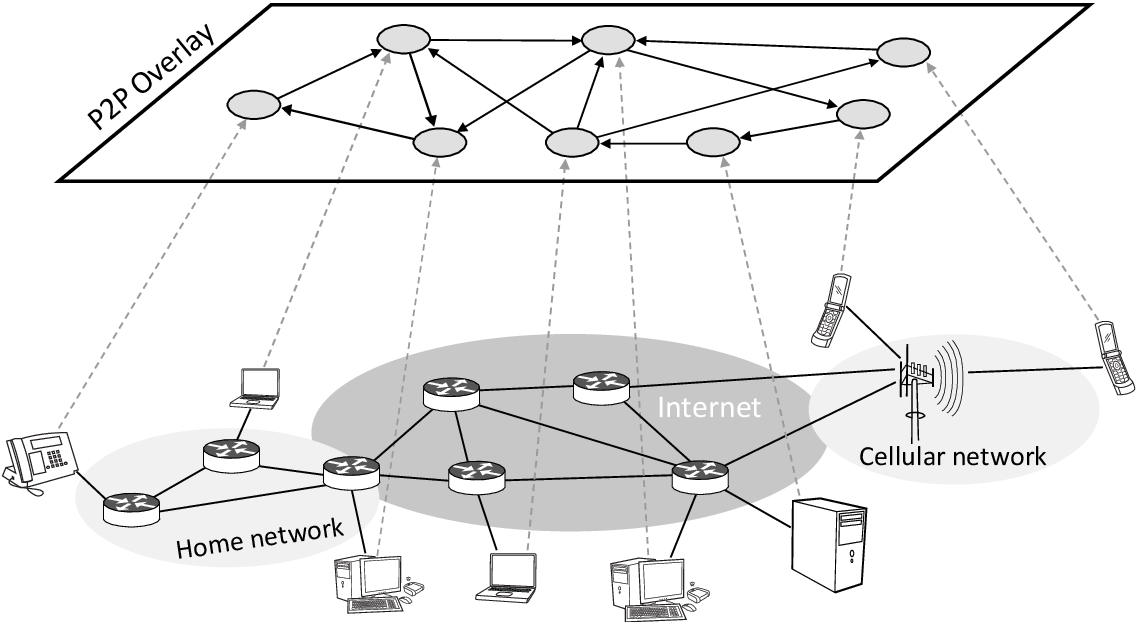
\includegraphics[width=0.9\linewidth]{images/overlay_network.png}
    \captionof{figure}{Peer-to-Peer-Overlay-Netzwerk mit darunterliegendem physischen Netzwerk \parencite{Kunzmann_OverlayNetworksImageSource}}
    \label{overlay_network}
\end{center}

\noindent In diesem Fall ist das physische Netzwerk das Internet. Das Overlay-Netzwerk ist eine logische Struktur, die es ermöglicht, die Kommunikation zwischen den Teilnehmern zu organisieren. Es besteht aus einer Reihe von Knoten, die über eine logische Verbindung miteinander verbunden sind. Die Verbindungen zwischen den Knoten werden durch Routing-Algorithmen verwaltet \parencite{Lua_P2POverlayNetworksPaper}.

Beispiele für diese Routing-Algorithmen sind \textit{Kademlia}, \textit{Chord} und \textit{Pastry}. Diese drei Algorithmen verwenden sogenannte \textit{Distributed Hash Tables} (zu Deutsch: \textit{Verteilte Hashtabellen}), um die Knoten zu verwalten. Distributed Hash Tables (kurz: \textit{DHTs}) sind verteilte Datenstrukturen, die in Peer-to-Peer-Netzwerken verwendet werden, um effizient Schlüssel-Wert-Paare zu speichern und abzurufen. Anders als herkömmliche zentralisierte Datenbanken oder Speicherlösungen, welche die Daten auf einem zentralen Server speichern, benötigen DHTs keinen solchen Server zur Speicherung oder Verwaltung der Daten. Sie funktionieren auf Basis von Hashfunktionen (siehe \ref{subsec:integritaet_signatur} \textit{\nameref{subsec:integritaet_signatur}}), die einen Schlüssel in einen eindeutigen Hash umwandeln. Diese Hashes dienen als Adressen, um zu bestimmen, wo die entsprechenden Daten im Netzwerk gespeichert sind. Die Daten werden über verschiedene Peers im Netzwerk verteilt, wobei jeder Peer nur einen Teil der Daten basierend auf seinem Verantwortungsbereich speichert. Diese Algorithmen ermöglichen es, Peers im Netzwerk zu finden, die für die Speicherung oder Abfrage von Daten zuständig sind, selbst wenn sich die Netzwerktopologie ständig verändert. Ein großer Vorteil von DHTs ist ihre Skalierbarkeit. Sie können mit der Netzwerkgröße wachsen, ohne an Effizienz zu verlieren. Neue Peers können nahtlos hinzugefügt werden, und die Struktur der DHT passt sich dynamisch an Veränderungen im Netzwerk an \parencites{Stoica_Chord}{Rowstron_Pastry}{Maymounkov_Kademlia}[S. 43-46]{Balakrishnan_LookingUpDataInP2PSystems}.


\subsection{Kademlia vs. Chord vs. Pastry}
\label{subsec:kademlia_vs_chord_vs_pastry}

\textit{Kademlia} ist ein Routing-Algorithmus, der auf einer k-Bucket-Struktur basiert. Das \textit{k} in k-Bucket steht für die Anzahl der Knoten, die in einem Bucket gespeichert werden können. Bei einem niedrigen Wert für \textit{k} reduziert den Aufwand, der benötigt wird, um eine Routing-Tabelle zu verwalten, aber erhöht das Risiko für das Versagen eines Knotens (engl. \textit{Node Failure}). Bei einem hohen Wert für \textit{k} ist es genau umgekehrt. Routing-Tabellen mit mehreren Buckets sind in der Lage, mehr (redundante) Knoten zu speichern, was das Routing sicherer vor Fehlern macht. Allerdings kostet die Verwaltung von mehr Buckets auch mehr Aufwand. Die Wahl eines geeigneten Wertes für \textit{k} ist daher entscheidend für die Leistungsfähigkeit, Fehlertoleranz und Skalierbarkeit des Netzwerks.Die gespeicherten Knoten werden in Buckets organisiert, wobei jeder Bucket für einen bestimmten Schlüsselbereich verantwortlich ist. Die Verbindungen zwischen den Knoten werden durch die XOR-Distanz der IDs definiert und sind asymmetrisch. Das bedeutet, dass ein Knoten  \textit{A} eine Verbindung zu einem anderen Knoten \textit{B} haben kann, aber deshalb \textit{B} keine Verbindung zu \textit{A} haben muss. Bei der Suche nach einem bestimmten Schlüssel erfolgt das Routing durch die XOR-Entfernung, wodurch die nächsten Knoten für diesen Schlüssel gefunden werden. Dieses Verfahren ermöglicht eine logarithmische Anzahl von Schritten für die Suche und bietet eine robuste Struktur, die gut mit dynamischen Netzwerkänderungen umgehen kann \parencite[S. 1-2]{Maymounkov_Kademlia}.

\textit{Chord} ist ebenfalls ein Routing-Algorithmus, basiert allerdings auf einer Ringstruktur. Die Knoten sind in einem Ring angeordnet und jeder Knoten ist für einen bestimmten Schlüsselbereich verantwortlich. Die Verbindungen zwischen den Knoten sind durch ihren Platz im Ring definiert, wobei jeder Knoten eine Verbindung zu seinem nächsten Nachbarn im Uhrzeigersinn hat. Bei der Suche nach einem bestimmten Schlüssel durchläuft eine Anfrage einen logarithmischen Pfad im Ring, wobei die Knoten auf dem Weg begrenzte Informationen über andere Knoten behalten, um Anfragen weiterzuleiten. Dieses Modell ist recht einfach und effizient für viele Anwendungsfälle, aber es könnte anfällig sein für Engpässe oder längere Suchzeiten, insbesondere wenn das Netzwerk dynamisch ist und sich die Konfiguration häufig ändert \parencite[S. 1-3]{Stoica_Chord}.

% #TODO: Pastry entfernen
\textit{Pastry} ist ein weiterer Routing-Algorithmus, der auf einer eindimensionalen Struktur basiert. Die Knoten sind in einem eindimensionalen Adressraum angeordnet, wobei jeder Knoten für einen bestimmten Schlüsselbereich verantwortlich ist. Die Verbindungen zwischen den Knoten werden durch eine gemeinsame Präfix-Länge definiert, wobei jeder Knoten eine Verbindung zu seinem nächsten Nachbarn hat. Jeder Knoten besitzt drei Listen: eine \textit{Routing-Tabelle}, eine \textit{Nachbarn-Liste} und eine \textit{Blatt-Liste}. Die Routing-Tabelle enthält Informationen über andere Knoten im Netzwerk, die für bestimmte Präfixe verantwortlich sind. Die Nachbarn-Liste enthält Informationen über die Knoten im Netzwerk, die am nächsten an diesem Knoten liegen. Die Blatt-Liste enthält Informationen über Knoten, die am nächsten und am weitesten von diesem Knoten entfernt sind. Dies hilft bei der Suche nach einem bestimmten Schlüssel, der nicht durch die Routing-Tabelle abgedeckt wird. Bei der Suche wird nach einem Knoten gesucht, der die größte Übereinstimmung im ID-Präfix besitzt. Dieser Knoten wird dann die Anfrage an den nächsten Knoten weiterleiten, der eine größere Übereinstimmung im ID-Präfix besitzt. Dieser Vorgang wird wiederholt, bis der Knoten gefunden wird, der für den Schlüssel verantwortlich ist. Dieses Verfahren ermöglicht eine logarithmische Anzahl von Schritten für die Suche und bietet eine gute Balance zwischen Effizienz und Skalierbarkeit \parencite{Rowstron_Pastry}.

Insgesamt bieten alle drei Algorithmen Lösungen für die mögliche Anwendung in einem Instant-Messaging-Kontext. Je nach Anwendungsfall können sie unterschiedliche Vorteile bieten. Kademlia ist gut geeignet für große, dynamische Netzwerke, Chord für statischere Netzwerke und Pastry für mittelgroße Netzwerke mit moderater Dynamik. Für den Anwendungsfall des Instant-Messaging ist die effektive Bewältigung von \textit{Churn} von entscheidender Bedeutung. Churn bezieht sich auf die häufigen Ein- und Austritte von Teilnehmern in einem Peer-to-Peer-Netzwerk. In einem Instant-Messaging Kontext bedeutet dies, dass Benutzer sich ständig anmelden oder abmelden. Ein Protokoll, das gut mit Churn umgehen kann, ist entscheidend, um eine zuverlässige und nahtlose Kommunikation zu gewährleisten. Das richtige Handling von Churn ist daher ein Schlüsselfaktor für die Leistungsfähigkeit und Stabilität eines Instant-Messaging-Protokolls \parencite[S. 316-317]{Peris_KademliaChurn}.


\subsection{Angriffe auf Peer-to-Peer-Netzwerke}

Peer-to-Peer-Netzwerke sind anfällig für verschiedene Arten von Angriffen. Diese Angriffe können in zwei Kategorien unterteilt werden: \textit{Angriffe auf die Integrität} und \textit{Angriffe auf die Verfügbarkeit}.

\subsubsection{Angriffe auf die Integrität}
\label{subsubsec:sybil_or_eclipse_attack_p2p}

Bei Angriffen auf die Integrität geht es darum, die Integrität der Daten zu gefährden, die im Netzwerk gespeichert sind. Ein Beispiel für einen solchen Angriff ist der \textit{Sybil-Angriff}. Bei diesem Angriff erstellt ein einzelner Angreifer mehrere Identitäten, um die Kontrolle über das Netzwerk zu erlangen \parencite[S. 251]{Douceur_SybilAttack}. Nach einer erfolgreichen Übernahme von Teilen des Netzwerks, besteht die Möglichkeit der Durchführung eines \textit{Eclipse}-Angriffs \parencite[S. 13-15]{Baptiste_AttacksOnP2PNetworks}. Bei einem \textit{Eclipse}-Angriff wird versucht, einen Peer von allen anderen Peers im Netzwerk zu isolieren. Dies wird erreicht, indem bereits durch den vorhergegangenen Sybil-Angriff die Mehrheit der Peers kontrolliert wird. Der Angreifer kann dann die Verbindungen des Opfers zu anderen Peers im Netzwerk verhindern, indem er die Verbindungen zu anderen Peers kontrolliert \Parencite[S. 14]{Baptiste_AttacksOnP2PNetworks}. 


\subsubsection{Angriffe auf die Verfügbarkeit}
\label{subsubsec:denial_of_service_attack_p2p}

Bei Angriffen auf die Verfügbarkeit geht es darum, die Verfügbarkeit des Netzwerks zu gefährden. Ein Beispiel für einen solchen Angriff ist der \textit{Denial-of-Service-Angriff}. Mit einem \textit{Denial-of-Service}-Angriff (kurz: \textit{DoS-Angriff}) wird versucht, die Verfügbarkeit eines Dienstes zu beeinträchtigen, indem die Ressourcen des Dienstes erschöpft werden, sodass diese ausfallen \parencite{Bicakci_DoSAttacks}. In einem Peer-to-Peer-Netzwerk kann ein DoS-Angriff auf verschiedene Arten durchgeführt werden. Eine Möglichkeit ist es, einen Peer mit Anfragen zu überfluten, um ihn zu überlasten. Eine andere Möglichkeit ist es, einen Peer mit gefälschten Informationen zu überfluten, um ihn zu täuschen. Beide Methoden führen dazu, dass der Peer nicht mehr in der Lage ist, seine Aufgaben zu erfüllen, was zu einem Ausfall des Dienstes führt. Dieser Angriff wird noch effektiver, wenn er von mehreren Angreifern gleichzeitig durchgeführt wird. Dies wird als \textit{Distributed Denial-of-Service}-Angriff (kurz: \textit{DDoS-Angriff}) bezeichnet. Bei einem DDoS-Angriff können mehrere Peers gleichzeitig mit Anfragen überflutet werden, was es schwieriger macht, den Angriff zu stoppen \Parencite[S. 6]{Baptiste_AttacksOnP2PNetworks}. Aber auch ein erfolgreicher Sybil-Angriff kann dazu führen, dass die Verfügbarkeit des Netzwerks gefährdet wird. Wenn ein Angreifer die Mehrheit der Peers kontrolliert, kann er die Verbindungen zu anderen Peers kontrollieren. Die Kommunikation zwischen den Peers kann dann durch falsches Routing verlangsamt oder auch ganz verhindert werden \parencite[S. 13]{Baptiste_AttacksOnP2PNetworks}.



